% Provenance (never printed): see sources/outline_sources.md (Year 2: metamorphic reactions,
% Clapeyron slopes, the Al2SiO5 diagram, the facies grid, protoliths). Definitions and facies
% table from the IUGS subcommission proposal (via the Granada translation); thermodynamic data
% from Robie and Hemingway (1995); experimental diagram from Holdaway and Mukhopadhyay (1993);
% curves from figdata/bachelor-2/facies.py; exercise and problem values in the Book 4 scratch
% calculator calc/ch10.py.
\chapter{Metamorphic Reactions and Facies}\label{ch:b2:metamorphic-facies}

A basalt that sinks with its plate does not stay a basalt. Its plagioclase and pyroxene
react, in the solid state, into other minerals, and the new assemblage depends on the
pressure and temperature it reached: a blue rock of glaucophane and lawsonite, or a
green-and-red rock of omphacite and garnet. Metamorphic rocks keep these minerals when
they return to the surface, and a petrologist who knows the reactions can read the
conditions back. This chapter writes those reactions with the thermodynamics of the
chemistry course, computes from measured data the most famous metamorphic phase diagram,
that of the three \ce{Al2SiO5} minerals, compares it with experiment, and organises the
assemblages of metamorphic rocks into facies.
% ledger: scmr:facies-assemblages

\begin{recall}
\textbf{From the high-school volume}: \omterm{def:b2:metamorphic-facies:metamorphism}{metamorphism}, metamorphic grade, index minerals
and isograds, contact \omterm{def:b2:metamorphic-facies:metamorphism}{metamorphism} and its aureole, foliation and schistosity,
lithostatic pressure; kyanite, andalusite and sillimanite as polymorphs, and their
phase diagram. \textbf{From the physics and chemistry books' Year 1 volumes}: the Gibbs
energy $G = H - TS$, whose minimum marks the stable state at given $T$ and $P$;
enthalpy, entropy and heat capacity; $\mathrm dG = V\,\mathrm dP - S\,\mathrm dT$; the
Clausius--Clapeyron relation for the vaporisation of a pure substance and the triple
point of water. \textbf{From the Year 1 volume}: subduction zones, collision belts and
the geotherm.
\end{recall}

\section{Metamorphism}\label{sec:b2:metamorphic-facies:metamorphism}

The high-school volume met \omterm{def:b2:metamorphic-facies:metamorphism}{metamorphism} as the transformation of a rock by heat and
pressure. An international recommendation gives the definition used here.

\begin{definition}[Metamorphism; protolith]\label{def:b2:metamorphic-facies:metamorphism}
\emph{Metamorphism}\index{metamorphism} is a process that changes the minerals or the
microstructure of a rock, or both, essentially in the solid state, as the rock adjusts
to physical conditions that differ from those under which it formed and from those
normally found at the Earth's surface and in the zone of diagenesis. It may coexist with
\omterm{def:b2:mantle-melting:melting}{partial melting} and may change the chemical composition of the rock. The rock before
metamorphism is its \emph{protolith}\index{protolith}.
\end{definition}
% ledger: scmr:metamorphism

The lower limit excludes diagenesis, the changes of a sediment as it is buried and
lithified, and the upper limit is melting, studied in \cref{ch:b2:crustal-melting}. The
agents are temperature, pressure, the fluids that circulate through the rock (water and
carbon dioxide above all) and deformation. \omterm{def:b2:metamorphic-facies:metamorphism}{Metamorphism} is classified by its extent and
its setting.
% ledger: scmr:metamorphism, scmr:types

\emph{Regional} \omterm{def:b2:metamorphic-facies:metamorphism}{metamorphism} affects large volumes of rock and goes with large-scale
tectonic processes: it is \emph{orogenic} in mountain belts, where crust thickens in a
collision; \emph{burial} \omterm{def:b2:metamorphic-facies:metamorphism}{metamorphism} affects rocks deeply buried under thick
sedimentary or volcanic piles, without deformation or magmatism, so that its rocks
usually lack schistosity; \emph{ocean-floor} \omterm{def:b2:metamorphic-facies:metamorphism}{metamorphism} alters the crust near
spreading ridges, where hot seawater circulates through it under steep thermal
gradients, and its recrystallisation is usually incomplete. \emph{Local} \omterm{def:b2:metamorphic-facies:metamorphism}{metamorphism}
has a local cause: \emph{contact} \omterm{def:b2:metamorphic-facies:metamorphism}{metamorphism} heats the country rocks of an intrusion;
\emph{hydrothermal} \omterm{def:b2:metamorphic-facies:metamorphism}{metamorphism} is driven by hot water-rich fluids;
\emph{dislocation} \omterm{def:b2:metamorphic-facies:metamorphism}{metamorphism}, in fault and shear zones, reduces the grain size and
makes mylonites and cataclasites; \emph{impact} \omterm{def:b2:metamorphic-facies:metamorphism}{metamorphism}, under a \omterm{def:b2:planet-formation-meteorites:fall-find}{meteorite} impact,
can melt and vaporise rock. \omterm{def:b2:metamorphic-facies:metamorphism}{Metamorphism} is called prograde while temperature rises and
retrograde while it falls.
% ledger: scmr:types

\section{Metamorphic reactions}\label{sec:b2:metamorphic-facies:reactions}

\begin{definition}[Metamorphic reaction; devolatilisation reaction]\label{def:b2:metamorphic-facies:reaction}
A \emph{metamorphic reaction}\index{metamorphic reaction} transforms a set of minerals
of a rock, the reactants, into another set, the products, in the solid state, possibly
with a fluid phase taking part. A \emph{devolatilisation reaction}\index{devolatilisation
reaction} is one that releases a volatile, water in a dehydration reaction or carbon
dioxide in a decarbonation reaction.
\end{definition}

Three types will appear in this chapter. Polymorphic changes, such as kyanite to
sillimanite or calcite to aragonite, keep the formula and change the structure.
Other reactions among solids redistribute components between minerals, such as
albite giving jadeite plus quartz:
\[
\ce{NaAlSi3O8 -> NaAlSi2O6 + SiO2}.
\]
\omterm{def:b2:metamorphic-facies:reaction}{Devolatilisation reactions} release a fluid, such as muscovite and quartz breaking down
at high temperature:
\[
\ce{KAl3Si3O10(OH)2 + SiO2 -> KAlSi3O8 + Al2SiO5 + H2O}.
\]
% ledger: day73:ms-qz

For a reaction among minerals of fixed composition, the change of Gibbs energy is
$\Delta_r G(T, P) = \sum G_{\text{products}} - \sum G_{\text{reactants}}$; the products
are stable where $\Delta_r G < 0$, the reactants where $\Delta_r G > 0$, and the two
coexist where $\Delta_r G = 0$.

\begin{definition}[Univariant reaction]\label{def:b2:metamorphic-facies:univariant}
A reaction among phases of fixed composition is \emph{univariant}\index{univariant
reaction} when its equilibrium condition $\Delta_r G(T, P) = 0$ leaves one variable
free: the equilibrium is a line in the pressure--temperature plane, which separates
the field of the reactants from that of the products.
\end{definition}

\begin{definition}[Clapeyron slope]\label{def:b2:metamorphic-facies:clapeyron}
The \emph{Clapeyron slope}\index{Clapeyron slope} of a reaction is the slope
$\mathrm dP/\mathrm dT$ of its equilibrium line in the pressure--temperature plane.
\end{definition}

\begin{proposition}[Clapeyron slope of a reaction]\label{prop:b2:metamorphic-facies:clapeyron}
Along the equilibrium line of a reaction with entropy change $\Delta_r S$ and volume
change $\Delta_r V$,
\[
\frac{\mathrm dP}{\mathrm dT} = \frac{\Delta_r S}{\Delta_r V}.
\]
\end{proposition}

\begin{proof}
For each phase $\mathrm dG = V\,\mathrm dP - S\,\mathrm dT$, so for the reaction
$\mathrm d(\Delta_r G) = \Delta_r V\,\mathrm dP - \Delta_r S\,\mathrm dT$. Along the line
$\Delta_r G = 0$ stays zero: $\Delta_r V\,\mathrm dP = \Delta_r S\,\mathrm dT$.
\end{proof}

This is the Clausius--Clapeyron relation of physics, written for solids. With
$\Delta_r S$ in \unit{J.mol^{-1}.K^{-1}} and $\Delta_r V$ in \unit{J.bar^{-1}} (one
\unit{J.bar^{-1}} is \qty{10}{cm^3}), the slope comes out in bars per kelvin. Two
consequences shape every metamorphic phase diagram. Among solids, entropy and volume
changes are small, so that a reaction line may be steep or shallow, positive or
negative: the high-temperature side holds the products of higher entropy, and the
high-pressure side those of smaller volume. In a \omterm{def:b2:metamorphic-facies:reaction}{devolatilisation reaction} the fluid
brings a large entropy, so the products lie on the high-temperature side; and the volume
of the fluid, large at low pressure and shrinking as pressure rises, makes the slope
shallow at low pressure and steeper at high pressure. The reaction line bends.
Experiments on muscovite and quartz place it at 603, 637 and \qty{662}{\celsius} at 1,
2 and \qty{3}{kbar} of water pressure: between 1 and \qty{2}{kbar} the line climbs
\qty{29}{bar} per kelvin, between 2 and 3, \qty{40}{bar} (\cref{exo:b2:metamorphic-facies:9}).
% ledger: day73:ms-qz

\section{The aluminosilicates}\label{sec:b2:metamorphic-facies:al2sio5}

\begin{definition}[Aluminosilicate polymorphs]\label{def:b2:metamorphic-facies:al2sio5}
The \emph{aluminosilicate polymorphs}\index{aluminosilicate polymorphs} are the three
minerals of formula \ce{Al2SiO5}: kyanite (triclinic), andalusite and sillimanite (both
orthorhombic).
\end{definition}
% ledger: rh95:al2sio5

They are common in metamorphosed mudstones, whose aluminium they carry, and since they
share a formula, which one grows depends only on pressure and temperature. The table
below gives their measured properties.

\begin{center}
\small
\begin{tabular}{@{}lrrrr@{}}
\hline
 & $\Delta_f H^\circ$ (\unit{kJ.mol^{-1}}) & $S^\circ$ (\unit{J.mol^{-1}.K^{-1}}) & $V^\circ$ (\unit{J.bar^{-1}}) & density (\unit{g.cm^{-3}})\\
\hline
kyanite & $-2593.8$ & 82.80 & 4.415 & 3.670\\
andalusite & $-2589.9$ & 91.39 & 5.152 & 3.145\\
sillimanite & $-2586.1$ & 95.40 & 4.986 & 3.250\\
\hline
\end{tabular}
\par\smallskip{\small Kyanite, andalusite and sillimanite at \qty{298.15}{K} and
\qty{1}{bar} (Robie and Hemingway, 1995); the enthalpies are uncertain by
\qty{2.0}{kJ.mol^{-1}}, the entropies by 0.5. Density from the molar mass,
\qty{162.046}{g.mol^{-1}}, and the volume.}
\end{center}
% ledger: rh95:al2sio5

Kyanite is the densest and has the least entropy: it is the high-pressure,
low-temperature polymorph. Andalusite, the least dense, holds low pressure; sillimanite,
of the highest entropy, holds high temperature. Their equilibrium lines can be computed.

\begin{method}[Computing a reaction line]\label{met:b2:metamorphic-facies:line}
(1) From the tables, form $\Delta_r H$, $\Delta_r S$ and $\Delta_r V$ at \qty{298.15}{K}
and \qty{1}{bar}. (2) Neglect the change of $\Delta_r H$ and $\Delta_r S$ with
temperature (heat capacities of products and reactants nearly equal) and of $\Delta_r V$
with pressure and temperature (solids barely compress or expand):
\[
\Delta_r G(T, P) \approx \Delta_r H - T\,\Delta_r S + \Delta_r V\,(P - 1).
\]
(3) Set it to zero: $P = 1 + (T\,\Delta_r S - \Delta_r H)/\Delta_r V$, a straight line of
slope $\Delta_r S/\Delta_r V$. (4) Where precision matters, replace $\Delta_r H$ and
$\Delta_r S$ by their values at temperature $T$, from tables of $H_T - H_{298}$ and $S_T$,
and solve again. (5) Keep only the part of each line where its two phases are more stable
than any third one.
\end{method}

For kyanite to andalusite, $\Delta_r H = \qty{3.9}{kJ}$, $\Delta_r S =
\qty{8.59}{J.K^{-1}}$ and $\Delta_r V = \qty{0.737}{J.bar^{-1}}$: at \qty{25}{\celsius}
and \qty{1}{bar}, $\Delta_r G = 3900 - 298.15\times8.59 = \qty{+1.34}{kJ}$, so kyanite,
not andalusite, is the stable polymorph at the Earth's surface; kyanite to sillimanite has
$\Delta_r G = \qty{+3.94}{kJ}$ there. The slopes are $8.59/0.737 = \qty{11.7}{bar/K}$ for
kyanite to andalusite, $12.60/0.571 = \qty{22.1}{bar/K}$ for kyanite to sillimanite and
$4.01/(-0.166) = \qty{-24.2}{bar/K}$ for andalusite to sillimanite, the only reaction of
the three whose high-temperature product is the less dense.
% ledger: rh95:al2sio5

\begin{definition}[Invariant point]\label{def:b2:metamorphic-facies:invariant}
An \emph{invariant point}\index{invariant point} is a point of the
pressure--temperature plane where three or more phases of a system coexist in
equilibrium and every \omterm{def:b2:metamorphic-facies:univariant}{univariant} line among them meets; no variable is free there.
\end{definition}

\begin{proposition}[The triple point]\label{prop:b2:metamorphic-facies:triple}
The three lines kyanite $=$ andalusite, kyanite $=$ sillimanite and andalusite $=$
sillimanite meet at one point. Around it, each line is stable on one side only; its
metastable extension lies in the field of the third polymorph.
\end{proposition}

\begin{proof}
For any $(T, P)$, $\Delta G_{\text{ky}\to\text{sil}} = \Delta G_{\text{ky}\to\text{and}} +
\Delta G_{\text{and}\to\text{sil}}$, since the Gibbs energies of andalusite cancel. Where
the first two lines cross, two of these terms vanish, so the third does too: the third
line passes through the crossing. Beyond the crossing, on the line kyanite $=$ andalusite,
say, $G_{\text{ky}} = G_{\text{and}}$, but the point lies on the sillimanite side of the
two other lines, so $G_{\text{sil}}$ is smaller than both: neither kyanite nor andalusite
is stable there, and the line is metastable.
\end{proof}

With the constant properties of the method, the triple point lies at
\qty{514}{\celsius} and \qty{3.88}{kbar} (the weekend problem); with the temperature
dependence of the tables, at \qty{536}{\celsius} and \qty{4.20}{kbar}. The experimental
diagram, built from reversed experiments, puts it at $504 \pm \qty{20}{\celsius}$ and
$3.75 \pm \qty{0.25}{kbar}$ (the figure below).
% ledger: rh95:al2sio5-ht, hm93:triple, hm93:table11

\begin{omfigure}
\centering
\begin{tikzpicture}
\begin{axis}[omrecord, width=0.84\linewidth, height=7.4cm,
  xmin=200, xmax=900, ymin=0, ymax=10, xlabel={$T$ (\unit{\celsius})}, ylabel={$P$ (\unit{kbar})},
  legend style={font=\scriptsize, at={(0.02,0.98)}, anchor=north west},
  tick label style={font=\scriptsize}, label style={font=\small}]
\addplot[very thick, blue!70!black] table[x=T_C, y=P_kbar] {figdata/out/bachelor-2-facies-stable-kyand.dat};
\addlegendentry{computed (tables)}
\addplot[thick, gray, densely dashed, mark=o, mark size=1.2pt] table[x=T_C, y=P_kbar] {figdata/out/bachelor-2-facies-hm93-kyand.dat};
\addlegendentry{experimental}
\addplot[thick, orange!85!black, mark=square*, mark size=1.3pt] table[x=T_C, y=P_kbar] {figdata/out/bachelor-2-facies-day73.dat};
\addlegendentry{muscovite + quartz}
\addplot[very thick, blue!70!black, forget plot] table[x=T_C, y=P_kbar] {figdata/out/bachelor-2-facies-stable-kysil.dat};
\addplot[very thick, blue!70!black, forget plot] table[x=T_C, y=P_kbar] {figdata/out/bachelor-2-facies-stable-andsil.dat};
\addplot[thin, blue!70!black, dashed, forget plot] table[x=T_C, y=P_kbar] {figdata/out/bachelor-2-facies-meta-kyand.dat};
\addplot[thin, blue!70!black, dashed, forget plot] table[x=T_C, y=P_kbar] {figdata/out/bachelor-2-facies-meta-kysil.dat};
\addplot[thin, blue!70!black, dashed, forget plot] table[x=T_C, y=P_kbar] {figdata/out/bachelor-2-facies-meta-andsil.dat};
\addplot[thick, gray, densely dashed, mark=o, mark size=1.2pt, forget plot] table[x=T_C, y=P_kbar] {figdata/out/bachelor-2-facies-hm93-kysil.dat};
\addplot[thick, gray, densely dashed, mark=o, mark size=1.2pt, forget plot] table[x=T_C, y=P_kbar] {figdata/out/bachelor-2-facies-hm93-andsil.dat};
\addplot[only marks, mark=*, mark size=2pt, blue!70!black, forget plot] table[x=T_C, y=P_kbar] {figdata/out/bachelor-2-facies-triple-B.dat};
\addplot[only marks, mark=*, mark size=2pt, gray, forget plot] table[x=T_C, y=P_kbar] {figdata/out/bachelor-2-facies-hm93-triple.dat};
\node[font=\small\bfseries] at (axis cs:330,6.2) {kyanite};
\node[font=\small\bfseries] at (axis cs:460,0.6) {andalusite};
\node[font=\small\bfseries] at (axis cs:790,3.6) {sillimanite};
\end{axis}
\end{tikzpicture}
\par\smallskip{\small The \ce{Al2SiO5} diagram computed from the thermodynamic tables of
Robie and Hemingway (1995) with temperature-dependent enthalpy and entropy (blue; dashed:
metastable extensions), and the experimental diagram of Holdaway and Mukhopadhyay (1993)
(grey, their tabulated points). Orange: the muscovite + quartz breakdown measured by
Day (1973), which bends.}
\end{omfigure}
% ledger: rh95:al2sio5, rh95:al2sio5-ht, hm93:table11, hm93:triple, day73:ms-qz

The computed kyanite--andalusite line falls within \qty{0.1}{kbar} of the experimental
one between 400 and \qty{600}{\celsius}, but the andalusite--sillimanite line lies
\qty{0.65}{kbar} too high at \qty{600}{\celsius}. That line is the most fragile of the
three: with $\Delta_r V = \qty{-0.166}{J.bar^{-1}}$, an error of \qty{0.1}{kJ} in
$\Delta_r H$, a twentieth of the uncertainty of each enthalpy in the table, moves it by
\qty{600}{bar}. The enthalpies of the tables are themselves adjusted to fit the
experiments, within their uncertainties; the experiments, not calorimetry alone, fix the
diagram.
% ledger: rh95:al2sio5, hm93:adjusted, hm93:table11

The figure below shows why a line is a boundary. At \qty{6}{kbar} the Gibbs energies of
andalusite and sillimanite, measured from that of kyanite, cross zero where each would
become more stable than kyanite; the differences never exceed a few kilojoules per mole,
which is why a small error in an enthalpy moves a line so far.

\begin{omfigure}
\centering
\begin{tikzpicture}
\begin{axis}[omrecord, width=0.7\linewidth, height=5.4cm,
  xmin=300, xmax=900, ymin=-4, ymax=4.5, xlabel={$T$ (\unit{\celsius})},
  ylabel={$G - G_{\text{kyanite}}$ (\unit{kJ.mol^{-1}})},
  legend style={font=\scriptsize, at={(0.02,0.02)}, anchor=south west},
  tick label style={font=\scriptsize}, label style={font=\small}]
\addplot[very thick, red!75!black] table[x=T_C, y=dG_and] {figdata/out/bachelor-2-facies-dg6.dat};
\addlegendentry{andalusite}
\addplot[very thick, green!45!black] table[x=T_C, y=dG_sil] {figdata/out/bachelor-2-facies-dg6.dat};
\addlegendentry{sillimanite}
\addplot[thin, black] coordinates {(300,0) (900,0)};
\end{axis}
\end{tikzpicture}
\par\smallskip{\small Gibbs energies of andalusite and sillimanite relative to kyanite at
\qty{6}{kbar}, from the same tables. Kyanite is stable while both curves are positive;
sillimanite takes over at \qty{624}{\celsius}. Andalusite crosses zero only at
\qty{692}{\celsius}, where sillimanite is already lower: above the pressure of the
triple point, andalusite is never the most stable.}
\end{omfigure}
% ledger: rh95:al2sio5, rh95:al2sio5-ht

\begin{inthelab}[Reversing a reaction]
A reaction line is located in the laboratory by experiments at fixed pressure and
temperature that start from a mixture of reactants and products. In a piston--cylinder
apparatus, the mixture is held for one to a few days; the direction of reaction is then
read from X-ray diffraction, by comparing the ratio of the peaks of product and reactant
with that of the starting mix, and confirmed by overgrowths on the stable mineral. Other
studies weigh a single crystal of andalusite reacted in a powder of kyanite or
sillimanite, with a microbalance precise to about \qty{4}{\micro g}. An equilibrium is
\emph{reversed} when growth of each side has been observed on either side of the line;
the line then lies in the bracket between, drawn with the errors of the apparatus,
typically \qty{10}{\celsius} and \qty{0.5}{kbar}. Experimenters judge a phase diagram first
by such reversals, and only second by the rocks.
\end{inthelab}
% ledger: hm93:methods

\section{Assemblages and facies}\label{sec:b2:metamorphic-facies:facies}

\begin{definition}[Mineral assemblage]\label{def:b2:metamorphic-facies:assemblage}
A \emph{mineral assemblage}\index{mineral assemblage} is the set of minerals that grew
together in equilibrium in a metamorphic rock.
\end{definition}

An assemblage depends on the conditions of \omterm{def:b2:metamorphic-facies:metamorphism}{metamorphism} and on the composition of the
rock. Eskola, who introduced the concept of facies in 1915, saw that rocks of the same
composition carry the same assemblage under the same conditions, and that the
assemblages of different rocks change together when the conditions change; the
international recommendation keeps his concept.
% ledger: scmr:facies

\begin{definition}[Metamorphic facies; facies grid]\label{def:b2:metamorphic-facies:facies}
A \emph{metamorphic facies}\index{metamorphic facies} is a set of metamorphic \omterm{def:b2:metamorphic-facies:assemblage}{mineral
assemblages}, repeatedly associated in time and space, showing a regular relationship
between mineral composition and bulk chemical composition, such that different facies
correspond to different metamorphic conditions, chiefly temperature and pressure. The
facies are named and defined on the assemblages of rocks of basaltic composition. A
\emph{facies grid}\index{facies grid} is the arrangement of the facies in the
pressure--temperature plane.
\end{definition}
% ledger: scmr:facies

The table below lists ten facies by their diagnostic minerals in metabasalts.

\begin{center}
\small
\begin{tabular}{@{}p{0.27\linewidth}p{0.66\linewidth}@{}}
\hline
facies & diagnostic minerals of a metabasalt\\
\hline
zeolite & zeolites such as laumontite and heulandite\\
prehnite--pumpellyite & prehnite + pumpellyite, prehnite + actinolite, pumpellyite + actinolite\\
greenschist & actinolite + albite + chlorite + epidote\\
epidote amphibolite & hornblende + albite + epidote $\pm$ chlorite\\
amphibolite & hornblende + plagioclase (more than \qty{17}{\percent} anorthite)\\
granulite & clinopyroxene + orthopyroxene + plagioclase; olivine not stable with plagioclase or garnet\\
blueschist & glaucophane + epidote $\pm$ garnet, or glaucophane + lawsonite\\
eclogite & omphacite + garnet; plagioclase not stable\\
pyroxene \omterm{def:b2:magma-emplacement:aureole}{hornfels} & clinopyroxene + orthopyroxene + plagioclase; olivine stable with plagioclase\\
sanidinite & the same, with very-high-temperature minerals such as pigeonite\\
\hline
\end{tabular}
\par\smallskip{\small The facies and their diagnostic assemblages in rocks of basaltic
composition, after the international recommendation (Eskola's eight facies, with the
zeolite and prehnite--pumpellyite facies added later).}
\end{center}
% ledger: scmr:facies-assemblages, scmr:facies

The recommendation stresses what the facies do not do: they record regularities among
assemblages, and do not try to fix the pressure and temperature of each. Their order in
the pressure--temperature plane follows from the reactions between them, and the
figure below draws it schematically. Temperature grows from the zeolite facies through
the greenschist and amphibolite facies to the granulite facies; at low pressure and high
temperature lie the \omterm{def:b2:magma-emplacement:aureole}{hornfels} facies of \omterm{def:b2:magma-emplacement:aureole}{contact aureoles}; at high pressure and low
temperature, the blueschist facies; at high pressure and higher temperature, the
eclogite facies. Reactions of this chapter fix pieces of the boundaries: plagioclase,
present as albite or as a more calcic plagioclase from the greenschist to the granulite
facies, is not stable in the eclogite facies, as its
albite does when it turns into jadeite and quartz (\cref{exo:b2:metamorphic-facies:8}); calcite turns into the
denser aragonite at high pressure (\cref{exo:b2:metamorphic-facies:7}).
% ledger: scmr:facies, scmr:facies-assemblages

\begin{omfigure}
\centering
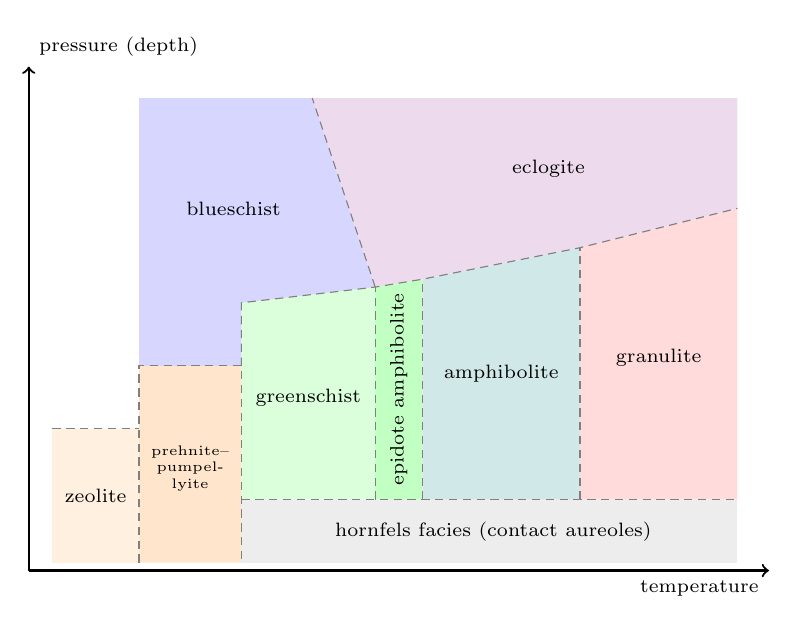
\begin{tikzpicture}[font=\scriptsize, x=1cm, y=1cm]
\draw[->, thick] (0,0) -- (9.4,0) node[below left] {temperature};
\draw[->, thick] (0,0) -- (0,6.4) node[above right] {pressure (depth)};
\fill[orange!12] (0.3,0.1) -- (1.4,0.1) -- (1.4,1.8) -- (0.3,1.8) -- cycle;
\fill[orange!20] (1.4,0.1) -- (2.7,0.1) -- (2.7,2.6) -- (1.4,2.6) -- (1.4,1.8) -- cycle;
\fill[green!14] (2.7,0.9) -- (4.4,0.9) -- (4.4,3.6) -- (2.7,3.4) -- cycle;
\fill[green!24] (4.4,0.9) -- (5.0,0.9) -- (5.0,3.7) -- (4.4,3.6) -- cycle;
\fill[teal!18] (5.0,0.9) -- (7.0,0.9) -- (7.0,4.1) -- (5.0,3.7) -- cycle;
\fill[red!14] (7.0,0.9) -- (9.0,0.9) -- (9.0,4.6) -- (7.0,4.1) -- cycle;
\fill[gray!14] (2.7,0.1) -- (9.0,0.1) -- (9.0,0.9) -- (2.7,0.9) -- cycle;
\fill[blue!16] (1.4,2.6) -- (2.7,2.6) -- (2.7,3.4) -- (4.4,3.6) -- (3.6,6.0) -- (1.4,6.0) -- cycle;
\fill[violet!14] (4.4,3.6) -- (5.0,3.7) -- (7.0,4.1) -- (9.0,4.6) -- (9.0,6.0) -- (3.6,6.0) -- cycle;
\draw[gray, densely dashed] (1.4,0.1) -- (1.4,2.6) -- (2.7,2.6) -- (2.7,0.1);
\draw[gray, densely dashed] (0.3,1.8) -- (1.4,1.8);
\draw[gray, densely dashed] (2.7,0.9) -- (9.0,0.9);
\draw[gray, densely dashed] (4.4,0.9) -- (4.4,3.6) (5.0,0.9) -- (5.0,3.7) (7.0,0.9) -- (7.0,4.1);
\draw[gray, densely dashed] (2.7,2.6) -- (2.7,3.4) -- (4.4,3.6) -- (5.0,3.7) -- (7.0,4.1) -- (9.0,4.6);
\draw[gray, densely dashed] (4.4,3.6) -- (3.6,6.0);
\node at (0.85,0.95) {zeolite};
\node[align=center, font=\tiny] at (2.05,1.3) {prehnite--\\pumpel-\\lyite};
\node at (3.55,2.2) {greenschist};
\node[rotate=90] at (4.7,2.3) {epidote amphibolite};
\node at (6.0,2.5) {amphibolite};
\node at (8.0,2.7) {granulite};
\node at (5.9,0.5) {hornfels facies (contact aureoles)};
\node at (2.6,4.6) {blueschist};
\node at (6.6,5.1) {eclogite};
\end{tikzpicture}
\par\smallskip{\small The \omterm{def:b2:metamorphic-facies:facies}{facies grid}, schematic: the order of the facies of the table in
the pressure--temperature plane. Boundaries are gradational and drawn without numbers on
purpose: the facies are defined by assemblages, and the reactions that bound them depend
on the composition of each rock.}
\end{omfigure}
% ledger: scmr:facies, scmr:facies-assemblages

\begin{omfigure}
\centering
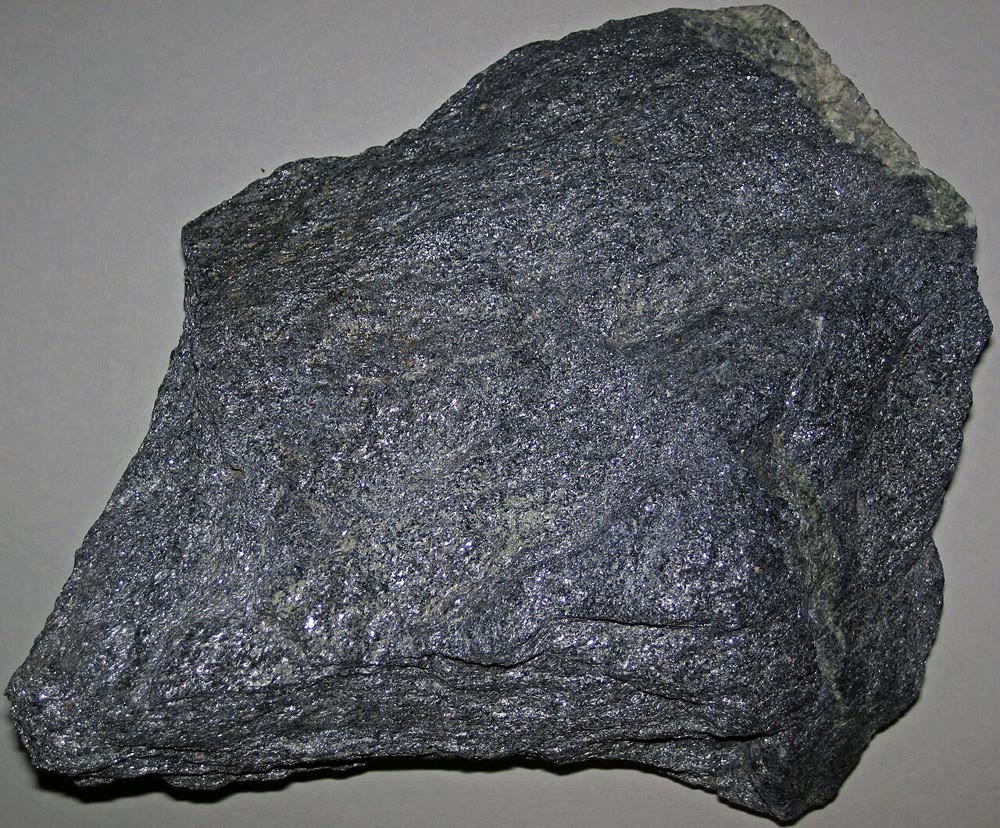
\includegraphics[width=0.27\linewidth]{images/book4/b2-10-blueschist.jpg}\hspace{0.02\linewidth}%
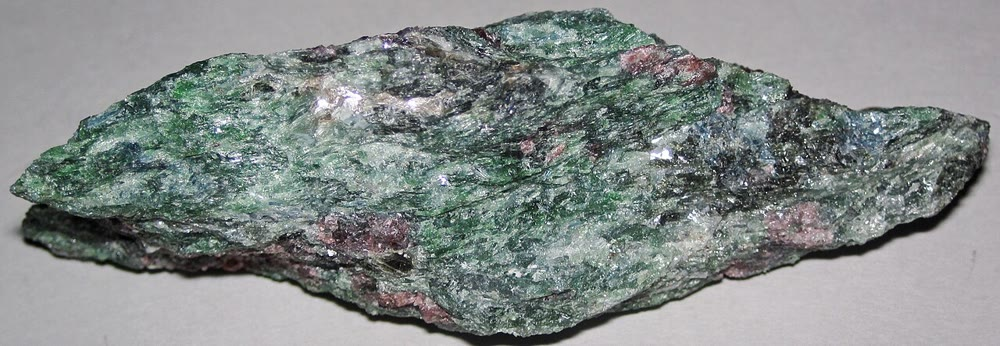
\includegraphics[width=0.69\linewidth]{images/book4/b2-10-eclogite.jpg}
\par\smallskip{\small Two metamorphosed basalts. Left: a lawsonite blueschist from the
Franciscan Complex of California, blue with glaucophane. Right: an eclogite from western
Norway, green omphacite and red garnet with some quartz, kyanite and rutile. Photographs
James St.~John, CC BY 2.0.}
\end{omfigure}

Rocks buried and heated together pass through facies in a regular order, which
reflects the ratio of pressure to temperature along their path: high in a subduction
zone, where blueschists form; intermediate in a collision belt; low near an intrusion.
\Cref{ch:b2:pt-paths} names these series and reads such paths from minerals.
% ledger: scmr:facies

\section{The protolith matters}\label{sec:b2:metamorphic-facies:protoliths}

The facies are defined on basalts, but every \omterm{def:b2:metamorphic-facies:metamorphism}{protolith} records the same conditions in
its own minerals.

\begin{definition}[Metapelite; metabasite]\label{def:b2:metamorphic-facies:protoliths}
A \emph{metapelite}\index{metapelite} is a metamorphosed mudstone (a pelite), rich in
aluminium and potassium, whose assemblages hold micas, chlorite, garnet, staurolite and
the aluminosilicates. A \emph{metabasite}\index{metabasite} is a metamorphosed basalt,
gabbro or other mafic rock, rich in calcium, magnesium and iron, whose assemblages define
the facies.
\end{definition}

In a \omterm{def:b2:metamorphic-facies:protoliths}{metapelite} the index minerals of the high-school volume appear in sequence as
grade rises (chlorite, biotite, garnet, staurolite, kyanite, sillimanite), the
muscovite + quartz reaction of this chapter makes sillimanite and K-feldspar at higher
temperature still, and the aluminosilicate present tells on which side of the triple
point the rock passed. A metamorphosed limestone or dolostone becomes a marble, of calcite or
dolomite; impure carbonates, with silica and clay, become calc-silicate rocks whose
decarbonation reactions release carbon dioxide; a quartz sandstone becomes a quartzite,
which shows little but its grain size. A \omterm{def:b2:metamorphic-facies:protoliths}{metapelite} of the chlorite zone and a
metabasalt beside it, at the same pressure and temperature, look nothing alike, the
second a greenstone of actinolite, chlorite, epidote and albite: one set of conditions,
two assemblages.
% ledger: iugs:barrow, day73:ms-qz, scmr:facies-assemblages

\section{Exercises}

\begin{exercise}[$\star$]\label{exo:b2:metamorphic-facies:1}
Name the type of \omterm{def:b2:metamorphic-facies:metamorphism}{metamorphism}: (a) a limestone recrystallised to marble within
\qty{500}{m} of a granite; (b) a fine-grained, banded rock along a large strike-slip
fault, its grains crushed and recrystallised; (c) a basalt of the ocean crust whose
glass has turned to chlorite and zeolites near a ridge, its minerals only partly
replaced; (d) volcanic sandstones at the bottom of a pile \qty{10}{km} thick,
recrystallised without schistosity.
\end{exercise}
% ledger: scmr:types

\begin{exercise}[$\star$]\label{exo:b2:metamorphic-facies:2}
From the table of the aluminosilicates, compute $\Delta_r S$, $\Delta_r V$ and the
\omterm{def:b2:metamorphic-facies:clapeyron}{Clapeyron slope} of kyanite $\to$ sillimanite, in \unit{bar/K} and in \unit{MPa/K}. By how
much does the equilibrium pressure change over \qty{100}{\celsius}?
\end{exercise}
% ledger: rh95:al2sio5

\begin{exercise}[$\star$]\label{exo:b2:metamorphic-facies:3}
To which facies does each metabasalt belong? (a) actinolite, albite, chlorite and
epidote; (b) glaucophane and lawsonite; (c) hornblende and plagioclase with
\qty{30}{\percent} anorthite; (d) omphacite and garnet, no plagioclase.
\end{exercise}
% ledger: scmr:facies-assemblages

\begin{exercise}[$\star$]\label{exo:b2:metamorphic-facies:4}
(a) From the molar mass \qty{162.046}{g.mol^{-1}} and the molar volumes 44.15, 51.52 and
\qty{49.86}{cm^3.mol^{-1}}, compute the densities of kyanite, andalusite and sillimanite.
(b) Which does pressure favour, and why? (c) Mineral databases give 3.61, 3.15 and
\qty{3.24}{g.cm^{-3}}: why can natural crystals differ from the pure phases?
\end{exercise}
% ledger: rh95:al2sio5, webmineral:polymorphs

\begin{exercise}[$\star\star$]\label{exo:b2:metamorphic-facies:5}
For kyanite $\to$ andalusite, $\Delta_r H = \qty{3.9}{kJ}$, $\Delta_r S =
\qty{8.59}{J.K^{-1}}$, $\Delta_r V = \qty{0.737}{J.bar^{-1}}$. (a) Which polymorph is
stable at \qty{25}{\celsius} and \qty{1}{bar}? (b) At what temperature do the two
coexist at \qty{1}{bar}? (c) Compute the equilibrium pressure at \qty{400}{\celsius} and
compare it with the experimental \qty{2.54}{kbar}. (d) Why is andalusite nonetheless
found in rocks that cooled to the surface?
\end{exercise}
% ledger: rh95:al2sio5, hm93:table11

\begin{exercise}[$\star\star$]\label{exo:b2:metamorphic-facies:6}
Test step (2) of the method. At \qty{1000}{K} the tables give $S_T$ = 285.02 for kyanite
and 296.44 for sillimanite, and $(H_T - H_{298})/T$ = 122.29 and 121.39
(\unit{J.mol^{-1}.K^{-1}}). (a) Compute $\Delta_r H$, $\Delta_r S$ and $\Delta_r G$ of
kyanite $\to$ sillimanite at \qty{1000}{K} and \qty{1}{bar}. (b) Compare with the constant
values of the table. (c) Which polymorph is stable there, and how large is the error of
the simple method?
\end{exercise}
% ledger: rh95:al2sio5-ht, rh95:al2sio5

\begin{exercise}[$\star\star$]\label{exo:b2:metamorphic-facies:7}
Calcite and aragonite (\ce{CaCO3}) have, at \qty{298.15}{K}, $\Delta_f G$ = $-1128.5$ and
$-1127.4$ \unit{kJ.mol^{-1}}, $S$ = 91.7 and 88.0 \unit{J.mol^{-1}.K^{-1}}, $V$ = 36.93
and \qty{34.15}{cm^3.mol^{-1}}, and equal enthalpies of formation. (a) Find the
equilibrium pressure at \qty{25}{\celsius}. (b) Compute the \omterm{def:b2:metamorphic-facies:clapeyron}{Clapeyron slope}. (c) Find the
equilibrium pressure at \qty{300}{\celsius}. (d) Many shells are made of aragonite and
live at \qty{1}{bar}: what does that say?
\end{exercise}
% ledger: rh95:cc-ar

\begin{exercise}[$\star\star$]\label{exo:b2:metamorphic-facies:8}
For albite $\to$ jadeite + quartz, the tables give $\Delta_r H = \qty{-5.0}{kJ}$,
$\Delta_r S = \qty{-32.4}{J.K^{-1}}$, $\Delta_r V = \qty{-1.698}{J.bar^{-1}}$. (a)
Compute the \omterm{def:b2:metamorphic-facies:clapeyron}{Clapeyron slope}. (b) Compute the equilibrium pressure at \qty{500}{\celsius}.
(c) The enthalpies of formation of albite, jadeite and quartz are uncertain by 2.6, 3.6
and \qty{1.0}{kJ.mol^{-1}}; combining them as independent errors, how uncertain is that
pressure? (d) Why does the eclogite facies lack plagioclase?
\end{exercise}
% ledger: rh95:ab-jd-qz, scmr:facies-assemblages

\begin{exercise}[$\star\star$]\label{exo:b2:metamorphic-facies:9}
Muscovite + quartz breaks down at 603, 637 and \qty{662}{\celsius} at 1, 2 and
\qty{3}{kbar}. (a) Compute the slope of the line between each pair of points. (b) If the
entropy of reaction hardly changes over this range, by what factor did $\Delta_r V$
shrink from the first interval to the second? (c) Which phase is responsible?
\end{exercise}
% ledger: day73:ms-qz

\begin{exercise}[$\star\star\star$]\label{exo:b2:metamorphic-facies:10}
With the constant properties of the method: (a) compute the pressures of the three
reactions at \qty{600}{\celsius}; (b) show that at \qty{600}{\celsius} and the pressure of
kyanite $=$ andalusite, sillimanite is the most stable polymorph, so that this point of
the line is metastable; (c) which polymorph is stable at \qty{600}{\celsius} and
\qty{4}{kbar}, and at \qty{600}{\celsius} and \qty{7}{kbar}?
\end{exercise}
% ledger: rh95:al2sio5

\begin{exercise}[$\star\star\star$]\label{exo:b2:metamorphic-facies:11}
A schist holds kyanite, andalusite and sillimanite together, all three grown in
equilibrium. (a) With the experimental triple point, $504 \pm \qty{20}{\celsius}$ and
$3.75 \pm \qty{0.25}{kbar}$, and a crust of density \qty{2700}{kg.m^{-3}} ($g =
\qty{9.81}{m.s^{-2}}$), at what depth did it grow? (b) Taking \qty{10}{\celsius} at the
surface, what mean thermal gradient does that imply? (c) Why are such rocks rare?
\end{exercise}
% ledger: hm93:triple

\begin{exercise}[$\star\star\star$]\label{exo:b2:metamorphic-facies:12}
Two rocks are buried to depth $z$, from \qty{10}{\celsius} at the surface: rock X along
\qty{10}{\celsius.km^{-1}} to \qty{30}{km} under rocks of mean density
\qty{3000}{kg.m^{-3}}, rock Y along \qty{30}{\celsius.km^{-1}} to \qty{20}{km} under rocks
of mean density \qty{2800}{kg.m^{-3}}. (a) Compute $T$ and $P$ at the end of each path.
(b) With the constant-property lines (calcite $=$ aragonite: $P = 13.31\,T$ bar with $T$
in kelvin; albite $=$ jadeite + quartz from \cref{exo:b2:metamorphic-facies:8}; the aluminosilicates from the
table), which of aragonite or calcite, of jadeite + quartz or albite, and which
aluminosilicate does each rock hold? (c) Which path is the colder, high-pressure one, and in which facies does each end?
\end{exercise}
% ledger: rh95:cc-ar, rh95:ab-jd-qz, rh95:al2sio5

\section{Problem: Building the triple point}

\begin{problem}[{Weekend problem --- the aluminosilicate diagram from the tables, and how
far to trust it}]
\label{pb:b2:metamorphic-facies:1}
Use the table of the aluminosilicates (\qty{298.15}{K}, \qty{1}{bar}) and the method of
this chapter, with constant $\Delta_r H$, $\Delta_r S$ and $\Delta_r V$; write $T$ in
kelvin, $P$ in bar, and neglect the 1 in $P - 1$.

\noindent\textbf{Part I --- The reactions.}
\begin{enumerate}
\item Compute $\Delta_r H$, $\Delta_r S$ and $\Delta_r V$ for kyanite $\to$ andalusite.
\item Do the same for kyanite $\to$ sillimanite.
\item Do the same for andalusite $\to$ sillimanite, and check that each property is the
difference of the first two.
\item Which polymorph has the largest entropy, which the smallest volume? On which side
of each line will each lie?
\item Compute the three \omterm{def:b2:metamorphic-facies:clapeyron}{Clapeyron slopes}.
\item Why is the slope of andalusite $\to$ sillimanite negative?
\end{enumerate}

\noindent\textbf{Part II --- Where the lines run.}
\begin{enumerate}[resume]
\item Compute $\Delta_r G$ of the first two reactions at \qty{298.15}{K}. Which
polymorph is stable at the surface?
\item At what temperature (in \unit{\celsius}) does each reaction reach equilibrium at
\qty{1}{bar}?
\item Of the three temperatures of question~8, which are stable equilibria and which
metastable? (Use the order of the three at \qty{1}{bar}.)
\item Compute the pressure of kyanite $=$ andalusite at \qty{400}{\celsius}; the
experiments give \qty{2.54}{kbar}.
\item Compute the pressure of kyanite $=$ sillimanite at \qty{700}{\celsius}; the
experiments give \qty{7.86}{kbar}.
\item Sketch the three lines between 200 and \qty{900}{\celsius}.
\end{enumerate}

\noindent\textbf{Part III --- The triple point.}
\begin{enumerate}[resume]
\item Write the first two lines as $P = a_i T - b_i$; give $a_1$, $b_1$, $a_2$, $b_2$.
\item Solve for the temperature of their intersection.
\item Compute its pressure.
\item Check that andalusite $=$ sillimanite passes through it.
\item Compare with the experimental $504 \pm \qty{20}{\celsius}$ and $3.75 \pm
\qty{0.25}{kbar}$.
\item With the temperature dependence of the tables, the triple point moves to
\qty{536}{\celsius} and \qty{4.20}{kbar}. Did the refinement bring it closer to
experiment? What does that suggest about the main source of error?
\end{enumerate}

\noindent\textbf{Part IV --- How far to trust it.}
\begin{enumerate}[resume]
\item Raise the enthalpy of formation of andalusite by \qty{1}{kJ}. By how much does
the kyanite $=$ andalusite line move in pressure, at fixed temperature?
\item By how much does the triple point move in temperature?
\item Do the same for a rise of \qty{1}{kJ} in the enthalpy of sillimanite.
\item Each enthalpy is uncertain by \qty{2.0}{kJ}. What range of triple-point
temperatures do the calorimetric data alone allow?
\item How, then, can thermodynamic tables reproduce the experimental diagram within
\qty{30}{\celsius}?
\item State the temperature of the triple point computed in Part III, rounded to the
degree: the key number of this problem.
\end{enumerate}
\end{problem}
% ledger: rh95:al2sio5, rh95:al2sio5-ht, hm93:triple, hm93:table11, hm93:adjusted
